\documentclass[11pt]{article}
\usepackage{fullpage}
\usepackage{amsmath}
\usepackage{spverbatim}
\usepackage{url}
\usepackage{enumitem}
\usepackage{CJK}
\usepackage{graphicx}
\graphicspath{ {images/} }

\usepackage[rightcaption]{sidecap}
\usepackage{wrapfig}

\begin{document}
\hspace{-1cm} \LARGE{\textbf{\textit{Phone Case that Dispenses Toiletries and Keys}}}

\LARGE{\textbf{\textit{}}}

\section*{Patent Number:}
\large{US4378565Z43}

\section*{Inventor:}
\large{Ankita Upadhyay}

\section*{Serial Number:}
\large{\verb|#| A1A13965Q}

\section*{Abstract:}
\large{This invention is a universal phone case that dispenses basic toiletries such as antibacterial wipes and breath strips. The phone case also contains a sliding component which can store up to two keys including a house key, mailbox key, etc. This invention is designed for those who fumble around their bags to reach for the items mentioned above but can never find them with ease. This is also made for those who tend to be forgetful and either lose or can't find their keys when necessary. This phone case would be slightly thicker than most phone cases and have a automated dispenser that the user can control by downloading an app. There would also be a manual unlocking option that the phone case owner could use to reach for the products if their phone dies. This would be done using a four-digit pin pad that would be on the bottom right corner on the back of the case.

The app would have a graphical user interface with options that users can choose from in terms of which item to dispense. There would be three slots on the left side of the phone case where the items would be dispensed. In terms of the items themselves, they must be thin enough to fit in the phone case and the right width to be extracted. The third slot would be reserved for the keys. The keys would slide out from the third slot and the user can select which of the two keys they want to use. In terms of the technology, this invention includes a graphical user interface for the apps and a mechanical shaft with notched disks that dispenses the specific toiletry/key. The graphical user interface would interact with the microprocessor, which translates electronic commands so that the hardware can execute them. 
}

\section*{Prior Art:}

\begin{itemize}

    \item \verb|[0001]| US 9852615 A. Publication Date: Dec 26, 2017. Filling Date: Sept 27, 2016. Jesus Perez. System and method for facilitating appliance control via a smart device
    
    \item \verb|[0002]| US 12327875 A. Publication Date: Oct 14, 2004. Filling Date: March 31, 2993. Michael Grannan. System and method for controlling appliances with a wireless data enabled remote control 
    
    \item \verb|[0003]| US 20090113478A1 A. Publication Date: Apr 30, 2009. Filling Date: Dec 4, 2008. Joseph Lee Haughawout. System and method for interacting with a program guide displayed on a portable electronic device
    
    \item \verb|[0004]| US 20100182236A1 A. Publication Date: Jul 22, 2010. Filling Date: March 29, 2010. Timothy Pryor. Compact rtd instrument panels and computer interfaces
    
\end{itemize}





\section*{Description:}

\nonindent \underline{Technical Field:} 
\begin{flushleft}
\verb|[0005]| 
\nonindent This invention includes an app with a graphical user interface that interacts with a microprocessor connected to the phone case hardware.

\verb|[0006]|
\nonindent The designated microprocessor then signals the phone case's internal disks to dispense the desired products. 

\verb|[0007]|
\nonindent There already exist phone cases that perform functions including, but not limited to lighting up and dispensing coffee. 

\end{flushleft}

\newline

{\setlength{\parindent}{0cm}\underline {Background:} 
\begin{flushleft}
\verb|[0008]| Phone cases these days serve as more than just protective covers for our cellular devices. There are wallet cases, light-up mirror cases, and even self-defense based cases that come with pepper spray. The one object most people reach for or use on a daily basis are phones. Many are also out and about with their lives and tend to forgo basic hygiene, which is why this invention will make staying sanitized and healthy easier. This patent is also designed for those who need a more convenient place to access their keys. Since there will be a slot for keys to be dispensed, In terms of the existing technology,  facilitating appliance control through a smart phone/device will allow this invention to have a solid foundation to build upon. Combining the automation capabilities of smart devices and the concept of multi-purpose phone cases paves way for this patent to provide value to people with busy lives who also want toiletries and key accessibility at their utmost convenience. 
\end{flushleft}

\newline

\nonindent \underline{Summary:} 
\nonindent\begin{flushleft}
\verb|[0009]| This invention includes mobile graphic user interface functionalities with a microprocessor that links to the notched disks in the mechanical shafts of the phone case to dispense the desired toiletries and keys. There is also a manual function to obtain the aforementioned items in case of system failure; this ensures accessibility and convenience at all times. Although the phone case might be slightly bulky, the ease of accessing hygiene positive items such as breath mints and hand sanitation wipes make the invention useful, practical, and applicable.
\end{flushleft}

\section*{Representative Drawing:}
\begin{figure}[h]
    \caption{Side view of slot dispenser}
    \centering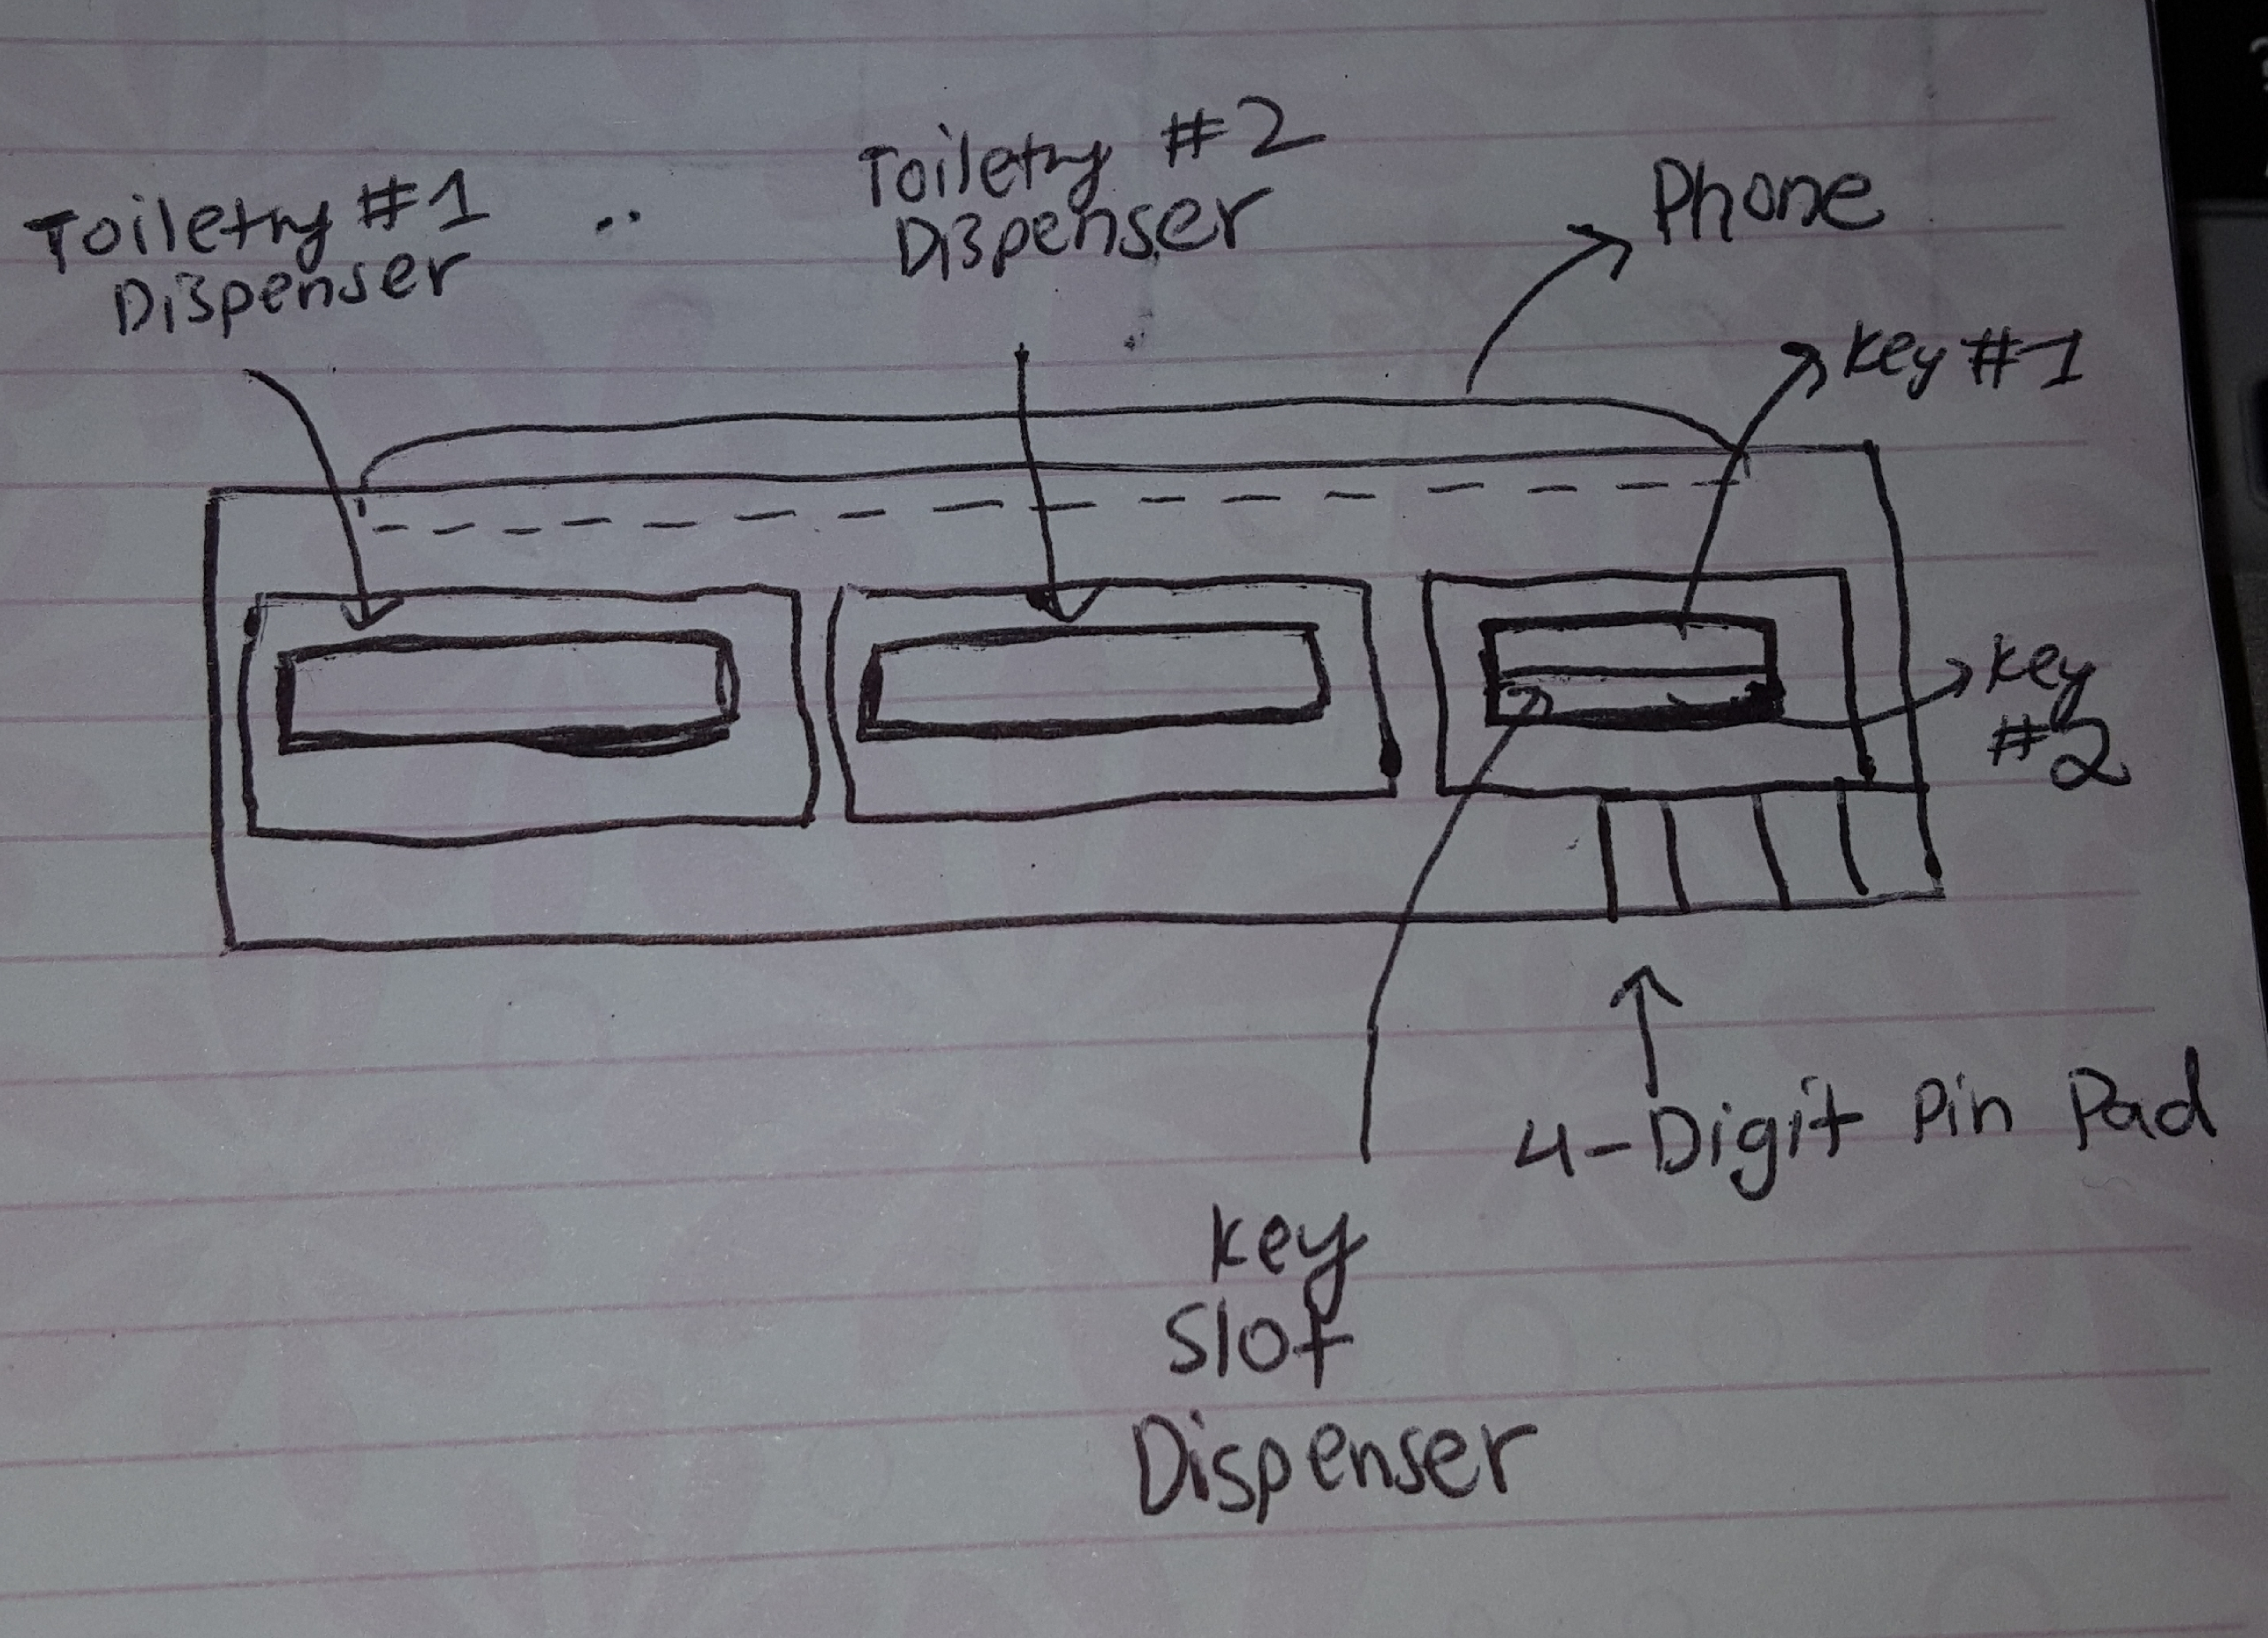
\includegraphics[height=6cm, width=8cm]{side.jpg}z
    \label{fig:design}
\end{figure}

\begin{figure}[h]
    \caption{Bird's eye view of phone }
    \centering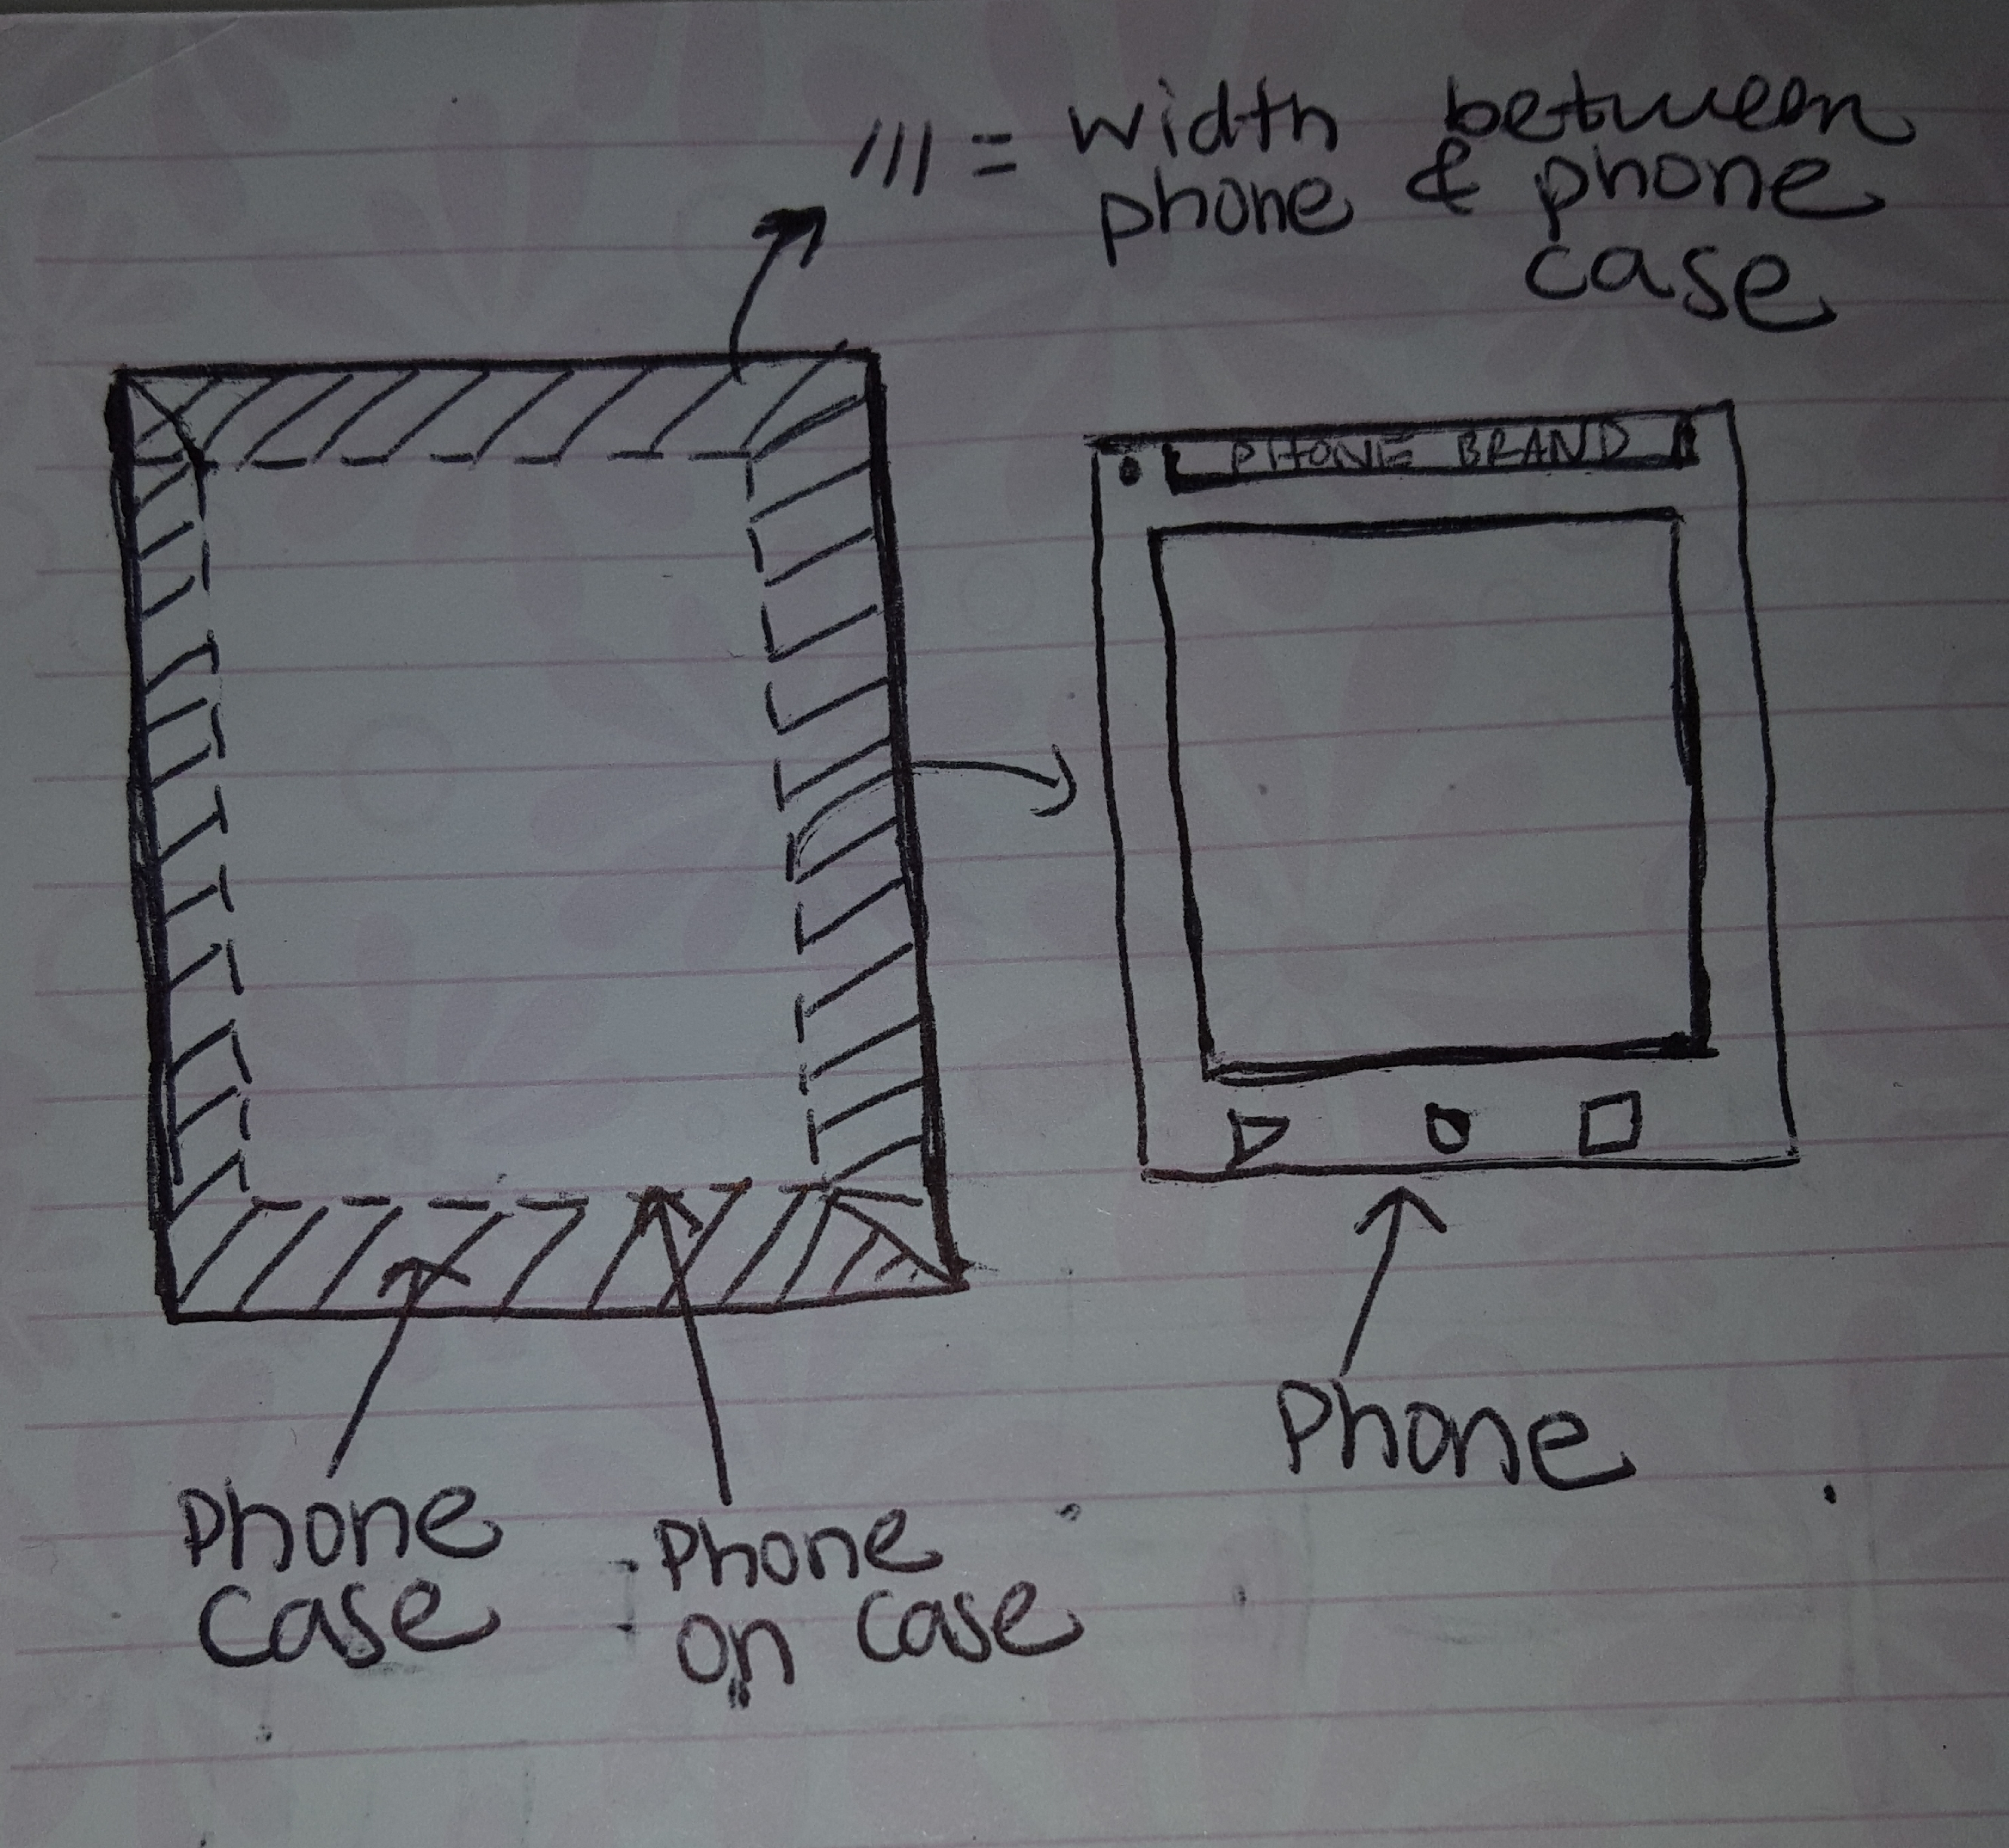
\includegraphics[height=6cm, width=8cm]{bird.jpg}
    \label{fig:design}
\end{figure}

\begin{figure}[h]
    \caption{Usage of the Drinking Vessel component fill-able from the Bottom and apparatus for dispensing a beverage therein PART 2}
    \centering\includegraphics[height=6cm, width=8cm]{holistic.jpg}
    \label{fig:design}
\end{figure}
\newpage



\newline
\newpage
\nonindent \underline{Figure 1 Description:} \verb|[0010]| This figure depicts the side view of the dispenser on the case and the corresponding toiletry/key slots.

\newline

\nonindent \underline{Figure 2 Description:} \verb|[0011]| This figure compares the placement/size of the phone case and the phone in terms of how they fit together.

\newline

\nonindent \underline{Figure 3 Description:} \verb|[0012]| This figure depicts the holistic view of the mobile app's graphical user interface and the internal phone case mechanisms in terms of the slots and the microprocessor status which signifies the status of slot dispensation (red equates to idle and green signals the said slot to dispense). 

\newline

\nonindent \underline{Detailed Description:} \verb|[0013]| 
When interacting with a mobile device, the user encounters a straightforward design of the app and can navigate through the different options by selecting any of the T1, T2, K1, or K2 slots. These slots indicate which item will be dispensed. Once chosen, the microprocessor will do its job by listening to the GUI commands and outputting the correct item. The K1 and K2 exist because the case allows the user to store up to two keys. The keys will then slide out and after using it, the user can simply slide it back in and lock it using the app. This ensures that the dispenser slot is secured and the key (or any other items) won’t fall out it it at any given time. The red and green lights represent active status and inactive status, respectively. Only one item can be dispensed at a time. When an item is being dispensed, the light will be green. This is under the phone case and is a part of the internal mechanism so the user will not be seeing the light status. 

\newline

\section*{Claims:} 

\begin{enumerate}
    \item {A graphical user interface controlled phone case that dispenses items, with a microprocessor, notched disks, and a four-digit pin pad, comprising:
        \begin{enumerate}[label=(\alph*)]
         an apparatus for dispensing essential toiletries stored with a phone case by selecting the desired items from the GUI of the app.
        \end{enumerate}
    }
    
    \item{The apparatus of claim 1, further comprising:
        \begin{enumerate}[label=(\alph*)]
        \item{corresponding slots that connect to the microprocessor,}
        \item{ a color coded status signal that indicates which slot to dispense}
        \item{the GUI of the app that commands the microprocessor to select the desired item to dispense}
        \end{enumerate}
    }
    
    \item{The corresponding slot part of claim 2, further comprising its capability to connect to the microprocessor that connects to the internal disk mechanisms.}
    
    \item{The color coded status part of claim 2, further comprising the signal to indicate slot availability,  such that in claim 3, the disk mechanisms correspond to the correct light status}
    
    \item{The software-hardware connectivity of claim 2, further comprising a microprocessor interaction with the graphical user interface.}
    
    \item{The graphical user interface of claim 5, further comprising the microprocessor to direct which specific item from which slot will be dispensed.}

    \item{The built-in product dispenser of claim 2, further comprising the user to use the app and select which specific toiletry or key they want to access}
    
    \item {The built-in product dispenser of claim 1, further comprising the use of the four-digit pin pad in case the mobile app does not function properly.}
    
\end{enumerate}

\end{document}

